\ifdefined\included
\else
\setcounter{chapter}{3} %% Numéro du chapitre précédent ;)
\dominitoc
\faketableofcontents
\fi

\chapter{Searching for a route with semantic knowledge}
\chaptermark{Searching for a route with an ontology}
\label{chap:3}
\minitoc

The contribution presented in this chapter is excerpted from our work, published in the proceedings of the Spatial Language Understanding (SpLU) 2019 workshop~\cite{sarthou_2019_semantic}. In this manuscript, the contribution is more detailed and discussed. This work is part of the MuMMER project, aiming at developing a robot guide in a mall. At the end of this thesis, a chapter is dedicated to the presentation of the project and the integration of the current contribution is a robotic system.

\section{Introduction}

We all have already been requested, or have ourselves request, for a route toward public space in a city, a shop in a shopping centre, or more simply a toilet in a house. When providing such information to a lost person we perform what is commonly called a guidance task. Even if it can seem evident for us, developing a robot able to perform it can be challenging. In this chapter, we choose to focus on the sub-task consisting to generate the explanation sentence. This sub-task is called the route description. To perform it, we first need a set of knowledge about the environment in which the guided person will walk, such as the paths, the intersections of the paths, or the elements alongside them. Then, we need a set of "good practices" to provide a route easy enough to follow and to remember.

In the Human-Robot Interaction (HRI) field, robots guides have been study intensively and deployed into shopping centers~\cite{okuno_2009_providing}, museums~\cite{burgard_1999_museum, clodic_2006_rackham, siegwart_2003_robox}, or airport~\cite{triebel_2016_spencer}. From a knowledge representation point of view, we can notice the use of metrical representations~\cite{thrun_2007_simultaneous} or topological representations~\cite{morales_2011_modeling} to represent the environment in which the robot evolves. Since we focus on the route description task, we consider that the robot does not accompany the human to his final destination but rather explains how to reach it. Consequently, the metrical representation will not be considered as being mainly used for navigation purpose~\cite{thrun_2007_simultaneous}. To perform more specifically a route description, topological knowledge is not sufficient. In addition to the topology of the environment, the robot needs to know the types of the elements composing the environment and their names in natural language. Some contributions have thus try to mix metrical or topological representations with semantic ones to hold this additional knowledge~\cite {satake_2015_should, chrastil_2014_cognitive, zender_2008_conceptual}. However, mixing them can create a lack of uniformity among the overall knowledge representation. In this way, creating a unique representation allowing a robot to compute routes and expressing them could ensure uniformity among the knowledge.

Even having a rich enough representation of its environment, the robot has to find a route not for it but for the guided human. A robot accompanying the human only has to determine a path, adapted to its capacities and interpretable only by it. Providing a route to a human, the route has to be adapted to the human capabilities. For example, in an outdoor environment, we will not give the same route for a car driver or a cyclist. In the context of a mall, we will not give a route with stairs along to a mobility-impaired person or to someone with a shopping cart. Once an adapted route computed, the robot has to explain. Where interactive maps only have to highlight a path, here, the robot has to generate a sentence that the human will memorize. For sure the robot will not instruct with a sentence like "walk 30 meters them turn -90 degrees". This would not be adapted to a human. The use of reference to the environment and orientation will be needed through a sentence like "walk until the florist then turn left".

The first contribution of this chapter is a unified representation of an indoor environment using an ontology to include both topological and semantic knowledge. Then, on the basis of this representation, we propose a first algorithm to find the suitable route to be explained to a human and a second algorithm to verbalize in an appropriate way.

First, we review the literature concerning indoor environment representation and route description. Then, we introduce the reader to our unified representation. We then present the algorithm used to compute the route and in a second time the algorithm to verbalize the previously computed route. We end this chapter with experimental results on both emulated and real environments.

\section{Related work}

\section{Representing indoor environment}

%Regarding the representation of the environment generally used in order to find an itinerary, we have first to analyse GNSS road navigation systems. In \cite{liu_route_1997} or \cite{cao_gps_2009}, we find the same principle of a topological network representing the roads with semantic information attached to each of them. This type of representation seems logical regarding the performance required for such systems operating in very large areas. However, GNSS road navigation systems must respond only to this unique task of finding a path when a robot is expected to be able to answer to various tasks. This is why we have developed and implemented a representation that can be used more widely while still allowing the search for routes.

%Morales et al. \cite{morales_building_2015} indicate that naming parts of a geometric map does not leave the opportunity to compute such perspective. As in \cite{satake_field_2015}, we have chosen to develop our representation with an ontology as it allows to reason about the meaning of words and thus improve the understanding of human demands. In addition, we propose a way to merge the topological representation into the semantic representation (the ontology) to get the meaning of the environment elements while keeping a description of the connectivity of the elements of the environment. We propose to name it semantic spatial representation (SSR). 

% More than the extension of the spatial semantic hierarchy (SSH) \cite{kuipers_spatial_2000} allowing the representation of the environment

%This paper focuses on the presentation of the SSR and on its usability for the route description task. For now, all the ontologies used to test the SSR have been made by hand. However, many recent research work leads to automatically generate a topological representation of an environment from geometric measurements (e.g. Region Adjacency Graphs \cite{kuipers_local_2004}, Cell and Portal Graphs \cite{lefebvre_automatic_2003} or hierarchical models \cite{lorenz_hybrid_2006}, or from natural language \cite{hemachandra_learning_2014}). We have not done it yet, but our system could benefit from this work to generate a representation of an environment using SSR, which would solve the complexity of creating such a representation by hand.


\section{Describing a route}

%In the literature, providing guidance is defined as a particular kind of spatial description called ``route description" or ``route directions". \cite{nishida_trading_2007}~defined it as a set of routes segment, each connecting two important points and explained in a chronological way. The way in which humans communicate spatial knowledge through the route description has been extensively studied both verbally and textually. This has allowed identifying invariants as well as good practices to ensure the success of the task in both urban and interior environments.
%Through five experiments, Allen~\cite{Allen_2000} identified three basic practices as important for communicating knowledge about routes. They can be summarized as follows: a) respect the spatiotemporal order, b) concentrate on the information about the points of choice and c) use landmarks that the listener can easily identify. This use of reference marks has been called critical information by Tversky in \cite{tversky_pictorial_1999} after highlighting that 91\% of the guidance contains additional information (landmarks) to the only actions of reorientation and directions \cite{tversky_how_1998}, which confirms the results of \cite{denis_description_1997}. Using the terms of \cite{Montello_1993}, guides usually used landmarks when the target places were no longer in the $Vista$ place (being within sight) but in the $Environmental$ space (being reachable through locomotion). In accordance with \cite{tversky_pictorial_1999}, using landmarks typically occurs when the explained action is a change of direction. In addition, the importance of landmarks and their choice based on salient features during a route description is described in \cite{nothegger_2004}.

%The choice of the route to explain may have an impact on its understanding and memorization: Morales in \cite{morales_building_2015} argued that the choice is based more on its complexity (the number of stages that compose it) than on its length.

%the three cognitive operations needed to generate a spatial discourse  \cite{denis_description_1997}: an activation of an internal representation of the environment;  the planning of a route in the mental representation made previously; the formulation of the procedure that the user must perform to achieve the objective.

%%% Aurélie: expliquer route perspective avec un exemple et montre la différence par rapport à l'autre perspective ?
%Route perspective means essentially to navigate mentally in order to verbalize the path to follow but also to facilitate understanding and memorizing instructions. The route perspective opposes the survey perspective which is a top view with landmarks and paths printed on a map. 

%With this, we are able to develop the two features presented in \cite{mallot_embodied_2009} for the route description task, which consist of selecting a sequence of places leading to the objective and managing the declarative knowledge to choose the right action to explain at each point of the sequence. Based on the principles of topological description, although represented semantically, we are able to compute multiple routes and new detours for the same objective in contrast with a route knowledge, which maps a predefined route to a given request. Thanks to this capacity and to the semantic knowledge of the environments available in the representation, it is also possible to provide the most relevant route to a user according to his preferences and capabilities. 

\section{The Semantic Spatial Representation}

\subsection{The SSR classes}

\begin{figure}[ht!]
\centering
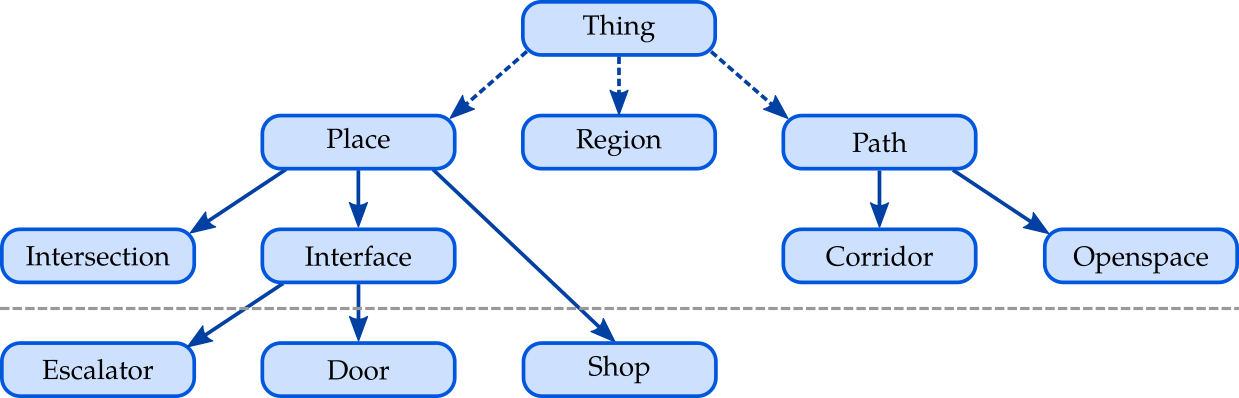
\includegraphics[scale=0.4]{figures/chapter3/ssr_tbox.png}
\caption{\label{fig:chap3_tbox} Representation fo the TBox (classes hierarchy) of the Semantic Spatial Representation used to describe the topology of an indoor environment. While the top part is inherent to the SSR, the bottom one extends the latter to provide more granularity.}
\end{figure}

\subsection{The SSR properties}

\begin{figure}[ht!]
\centering
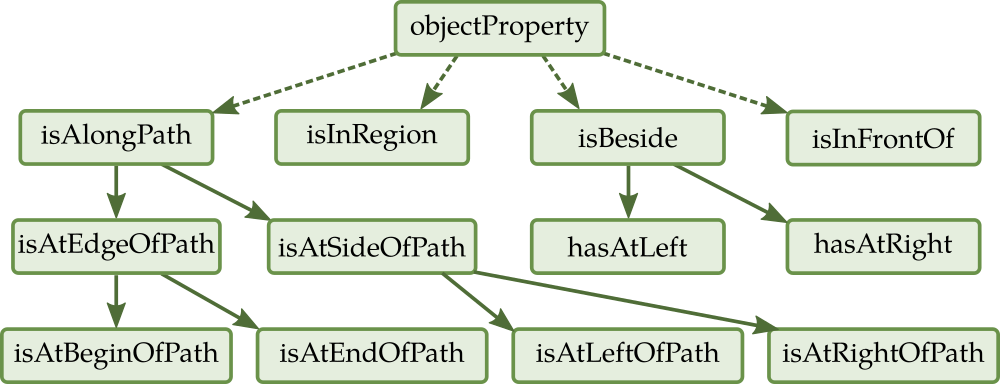
\includegraphics[scale=0.4]{figures/chapter3/ssr_rbox.png}
\caption{\label{fig:chap3_rbox} Representation fo the RBox (properties hierarchy) of the Semantic Spatial Representation used to describe the topology of an indoor environment.}
\end{figure}


\section{Finding routes to the right destination: A two-level search}

\subsection{The region-level: Trim down the search}

\begin{figure}[ht!]
\centering
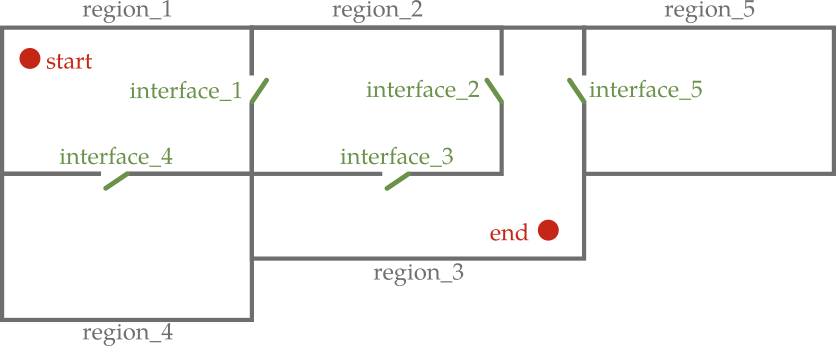
\includegraphics[scale=0.55]{figures/chapter3/regions.png}
\caption{\label{fig:chap3_regions} Representation of an environment at the region-level. Regions are linked trhough interfaces. We know that the starting point of the search is in \textit{region\_1} and the goal place is in \textit{region\_3}. }
\end{figure}


\subsection{The place-level: Refine the search}

\subsection{Selecting the most suitable route}

\section{Genarating an explanation in natural language}

\subsection{Putting the robot in your shoes}

\subsection{A pattern-based generation}

\section{Experiment in emulated and real environment}



